\documentclass[
   catalan,
   handout,
   ]{beamer}
\usepackage{babel}
\usepackage[utf8]{inputenc}
\usepackage[style=authoryear,sortcites=true]{biblatex}
\newcommand{\bibendash}{--}
\usepackage{cclicenses}
\usepackage{appendixnumberbeamer}
\usepackage{tikz}
\usetikzlibrary{shapes,arrows,positioning}
\usepackage{pgfplots}
%\usetikzlibrary{dateplot}  
%\usetikzlibrary{pgfplots.groupplots}






% \pgfplotsset{
%    rrbtimeseries/.style={
%         % date coordinates in=x,
%         ylabel=Temperature (K),
%         % legend style={font=\footnotesize},
%         % tick label style={font=\footnotesize},
%         % every axis x label/.style={
%         %   at={(1.3,0)},
%         %   anchor=north,
%         %   },
%         % label style={font=\footnotesize},
%         % xticklabel style= {rotate=17,anchor=north east},
% %        every axis title shift=0pt,
% %        max space between ticks=15,
%        %  every mark/.append style={mark size=6},
%        %  major tick length=0.1cm,
%        %  minor tick length=0.066cm,
%        %  very thin,
%        %  every axis legend/.append style={
%        %    at={(1.2,0)},
%        %    anchor=south east,
%        %    draw = none},
%        % legend columns = 4,
%        % unbounded coords=jump, %v>1.4
%     },

%   % rrbrs/.style={
%   %       rrbtimeseries,
%   %       width = \textwidth,
%   %       height = 0.25\textwidth,
%   %       every axis x label/.style={
%   %         at={(1.3,-1)},
%   %         anchor=north,
%   %         },
%   %       ylabel = {},  
%   %       max space between ticks=50,
%   %       every axis legend/.append style={
%   %         at={(1,-1.1)},
%   %         anchor=north east,
%   %         draw = none},
%   %       title style={font=\small,below,anchor=north,fill=white},
%   %   },
%  }




\pgfplotsset{
   timeseries/.style={
%        date coordinates in=x,
        ylabel=Temperature (K),
        legend style={font=\footnotesize},
        tick label style={font=\footnotesize},
        every axis x label/.style={
          at={(1.3,0)},
          anchor=north,
          },
        label style={font=\footnotesize},
        xticklabel style= {rotate=17,anchor=north east},
%        every axis title shift=0pt,
%        max space between ticks=15,
        every mark/.append style={mark size=6},
        major tick length=0.1cm,
        minor tick length=0.066cm,
        very thin,
        every axis legend/.append style={
          at={(1.2,0)},
          anchor=south east,
          draw = none},
       legend columns = 4,
    },
    rd/.style={
        timeseries,
        % every axis x label/.style={
        %   at={(1.3,-1)},
        %   anchor=north,
        %   },
        label style={font=\footnotesize},
        ylabel = {},
        width=\textwidth,
        height=3.5cm,   
        max space between ticks=50,
        every axis legend/.append style={
          at={(1,-1.1)},
          anchor=north east,
          draw = none},
%        title style={font=\small,below, at={(0.7,1.7)},anchor=north},
    }
}


%        unbounded coords=jump, %v>1.4
%        unbounded coords=discard, %v>1.4


%http://tex.stackexchange.com/questions/46422/axis-break-in-pgfplots

%http://tex.stackexchange.com/questions/52409/insert-a-separate-mark-inside-a-pgfplots-graph
\usetikzlibrary{dateplot}

\mode<beamer>
{
  \usetheme{Madrid}
  \useoutertheme[subsection=false]{smoothbars}
  \setbeamercovered{transparent}
  \beamertemplatenavigationsymbolsempty
}

\mode<handout>
{
  \usepackage{pgfpages}
  \pgfpagesuselayout{2 on 1}[a4paper,border shrink=5mm]
  %\pgfpagesuselayout{8 on 1}[a4paper,border shrink=5mm]
  \setbeamercolor{background canvas}{bg=black!5}
  \usetheme{Madrid}
  \useinnertheme{default}
  \usecolortheme{dove}
}


% \makeatletter
% \patchcmd{\slideentry}
% {}%{\advance\beamer@tempdim by -.05cm}
% {}%{\advance\beamer@tempdim by\beamer@vboxoffset\advance\beamer@tempdim by\beamer@boxsize\advance\beamer@tempdim by 1.2\pgflinewidth}
% {}
% {}
% \patchcmd{\slideentry}
% {}%{\kern\beamer@tempdim}
% {}%{\advance\beamer@tempdim by 2pt\advance\beamer@tempdim by\wd\beamer@sectionbox\kern\beamer@tempdim}
% {}
% {}
% \makeatother


\bibliography{../bibliografia}
\renewcommand*{\bibfont}{\footnotesize}
\bibparsep 0.2cm
\bibhang 0.25cm
%\ExecuteBibliographyOptions{
%  isbn=false,url=false,doi=false,firstinits=true,abbreviate=true
%}


%------------- capçaleres pdf -----------

\title%
   [Model multiresolució per a sèries temporals]%
   {Disseny i modelització d'un sistema de gestió multiresolució per a sèries temporals}

\author[A. Llusà]
{%
  Aleix Llusà Serra \\
  {\footnotesize Direcció: Teresa Escobet Canal i Sebastià Vila-Marta}
}

\institute[Programa doct.\ ARV UPC]
{
  {\large Universitat Politècnica de Catalunya} \\
  Programa de Doctorat en Automàtica, Robòtica i Visió 
}


\date[Desembre 2015]
{Tesi Doctoral \\ Desembre 2015}


\subject{Defensa de tesi doctoral 2015}
\keywords{sèries temporals; model de dades; sistemes de bases de dades; sistemes de monitoratge}



\begin{document}

\begin{frame}[plain]
 \titlepage

 \begin{center}
   {\footnotesize \cc\bysa}
   {\tiny Aquest document està sotmès a una llicència de Reconeixement-CompartirIgual 3.0 de Creative Commons\\
     El codi font \LaTeX\ del document es troba a
     \url{http://escriny.epsem.upc.edu/projects/rrb/} }
  \end{center}

\end{frame}

\section*{Índex}
\begin{frame}{Índex}
 \tableofcontents
\end{frame}


\section{Introducció}
\begin{abstract}
  Current monitoring systems are an essential part of supervising
  control as they manage a large amount of information. Data
  collection is normally studied as a time series owing to it fits
  into sequence of values.  Thanks to the facility of designing
  monitoring hardware, the measurement of data has increased the last
  decade and there is not enough capacity to store nor process all the
  time series. Therefore, we need to design database management
  systems capable of storing and processing efficiently the time
  series. Moreover, this systems have to cope with the measurements
  not happening at regular time intervals as it is a restriction
  imposed by some time series treatment algorithms.

  In this paper a formal model for a time series database management
  system is designed.  It is called Multiresoltion Time Series
  Database Management Systems model (MTSMS). A Time series is
  compactly stored in the database and the information is summarised
  by different interpolation functions. From this model this kind of
  DBMS will be better understood, new implementations will be possible
  and we will be able to enhance its potential.
\end{abstract}



\section{Introduction}

This paper focuses on Data Base Management Systems (DBMS) that store
and treat data as time series.  Traditional DBMS, as is ones derived
from relational model, are not adequate for these cases as they do not
have enough facilities to manage and retrieve time series
information \parencite{schmidt95}.

Some DBMS have already taken into account the specificities of time
series, then called Time Series Data Base Management Systems
(TSMS) \parencite{dreyer94}.  Time Series Data
Server \parencite{weigel10} allows to select a data range from a time
series and to apply a filter when the data is retrieved.
RRDtool \parencite{rrdtool} applies filters and stores different data
ranges when data is stored, moreover it considers that the sampling
times can not be equally spaced, the temporal order is essential and
the value and time must be stored together. However, this TSMS lack
the complete definition of the relation between the three main fields
involved: time series, monitoring systems and DBMS.

Monitoring sensor data and processing this data to achieve diagnosis,
prognosis, prediction, data fusion or other time series analysis tasks are common in many fields such as prognosis in degradation models \parencite{yu11}, qualify sensor health in navy vessels \parencite{palmer07}, validate and reconstruct data in water distribution networks \parencite{quevedo10}, sensor networks information dissemination \parencite{deligiannakis07} or economic stock classification \parencite{dreyer95}. Time series data mining formalises the knowledge discovery in time series databases \parencite{last01}. 


DBMS are based from formal models that define the objects and
operations of the abstract machine to which users interact, such is
the relational model \parencite{date}. TSMS lack a consolidated formal
model, although special properties and requirements for a TSMS
have been proposed \parencite{dreyer94}.

In this paper
a model is proposed for an storage system that will keep a time series
in a multiresolution and bounded way.  In this first proposal there
are six definitions that are related to the data storage mechanism:
measure, time series, buffer, disc, resolution disc, and multiresolution
database. Some of this concepts are familiar with RRDtool
operating mode.


\todo{estructura article}
The paper is organised as follows. In \autoref{sec:preliminaries} the preliminaries concerning TSMS are summarised. In \autoref{sec:TSMS} the state of TSMS is shown as well as known similar systems that are designed with some TSMS properties. In \autoref{sec:MTSMS} a model for a multiresolution TSMS is presented for the first time. Possible reference implementations of this model are explored in \autoref{sec:implementation}. In sections \ref{sec:conclusion} and \ref{sec:future}  the MTSMS is concluded and future work is proposed. In \autoref{sec:notation} the main nomenclature and notation used in the paper is summarised. 




%%% Local Variables: 
%%% mode: latex
%%% TeX-master: "article"
%%% ispell-local-dictionary: "british"
%%% End: 



\section{Formalització dels models}
\begin{frame}{Formalització dels models}

  \begin{enumerate}
  \item Sistemes de gestió de sèries temporals (SGST)
  \item Exemple de multiresolució
  \item Sistemes de gestió de sèries temporals multiresolució (SGSTM)
  \end{enumerate}

\end{frame}

\chapter{Model SGST}

En aquest capítol es defineixen els objectes que ens permeten modelar l'estructura de les dades.

Dos models estructurals:

* Hi ha un model pels SGST (TSMS) que inclou mesura i sèries temporals.

* Hi ha un model pels SGSTM (MTSMS) que té buffer, discs i mtsdb, els quals inclouen el model de sèrie temporal del SGST.




\section{Model estructural de dades}

Una sèrie temporal és una relació de temps i valors. A cada parella
temps-valor l'anomenem mesura. Així doncs, una sèrie temporal és un
conjunt de mesures. Una mesura és un tuple temps-valor.



Una mesura és un valor mesurat en un instant de temps i una sèrie
temporal és un co\l.lecció de mesures.





\subsection{Temps}

Utilitzem el temps com un valor que ens permet ordenar les mesures.  A
tal efecte, el domini del temps es defineix com un conjunt tancat
(compactificat) i amb ordre total. No obstant, pot ser tant un conjunt
finit com infinit.

Per facilitar la comprensió, en el document utilitzarem el conjunt de
reals com a conjunt pels temps. Concretament, per a complir que sigui
un conjunt tancat usarem el conjunt estès de nombres reals
$\bar{\mathbb{R}} \in \mathbb{R} \cup
\{+\infty,-\infty\}$, \parencite{wiki:extendedreal,cantrell:extendedreal},
també anomenat recta real acabada.


El conjunt estès de nombres reals té dos punts límits corresponents al
valor impropi infinit, aleshores en notació d'interval el conjunt es
pot escriure com $\bar{\mathbb{R}} \in [-\infty,+\infty]$.  Més
endavant a la definició~\ref{def:model:mesura_indefinida} es detallen
algunes propietats induïdes a les mesures com a resultat d'aquesta
extensió.

Les relacions d'ordre i algunes operacions aritmètiques s'estenen al
conjunt $\bar{\mathbb{R}}$, \cite{cantrell:extendedreal}.  Algunes
expressions esdevenen indefinides (p.ex.\ $0/0$) i altres depenen del
context, com és el cas de l'expressió indeterminada $0 \times \infty$ que
per exemple en la teoria de la mesura habitualment es defineix com $0 \times
\infty = 0$, \cite{wiki:extendedreal}.


El conjunt dels reals és un espai mètric ja que té definida una funció
distància (o mètrica), com per exemple la distància euclidiana. Com a
conseqüència, ens permet distingir entre instants de temps (els
elements del conjunt) i durades (la mètrica). Observant els instants
de temps com a punts en la recta real i les durades com a segments de
la recta real, es pot definir el temps com a sistema de coordenades
especificant un instant com a marc de
referència, \parencite{iep:time-supplement,wiki:coordinate}.


\begin{definition}[Temps]
  \label{def:model:temps}
  Siguin $t^i_i$ i $t^i_j$ dos instants de temps, observem la quantitat
  de temps o la durada $t^d$ com un valor $t^d \in\bar{\mathbb{R}}$
  que mesura la distància en unitats de temps entre dos temps
  absoluts $t^d = t^i_i - t^i_j$.
  
  Sigui $t^d$ una durada i $t^{R}$ un temps absolut de referència,
  observem un instant de temps $t^i$ com un valor $t^i
  \in\bar{\mathbb{R}}$ que mesura la quantitat de temps respecte al
  temps de referència $t^i= t^{R} + t^d$ . Aquest valor de referència
  $t^{R}\in\mathbb{R}$ és també un instant de temps però que permet
  definir unívocament la posició de qualsevol altre instant de temps.


\end{definition}

En resum, els instants de temps es poden veure com una seqüència de
valors reals que indiquen esdeveniments amb ordre clarament definit i
entre dos instants de temps sempre hi ha una durada. Tant els instants
de temps com les durades s'expressen amb un real que té unitats de
temps. Aquestes unitats són 'segons' en sistema internacional.



\subsubsection{Calendari}
\textcite{dreyer94} situen els calendaris i les seves operacions com a
essencials en els SGST. Tanmateix, pot no ser necessari modelar les
dates de calendari en el model de temps. El temps és la línia contínua
de temps, el calendari són nom especials a certs punts de la línia de
temps. Només cal una eina que sigui capaç de convertir de noms a
instants de temps.

Per una banda, no afecta al model SGST que els calendaris siguin més o
menys complicats, en aquest cas només es veuen complicades les
funcions de conversió de temps a calendari i viceversa.  Per altra
banda, tampoc afecta que els calendaris siguin ambigus (p.ex.\ dos
noms per al mateix instant o instants sense nom) o que continguin
propietats impredictibles (p.ex.\ cas dels segons addicionals
(intercalats) en UTC) ja que la responsabilitat d'aquests problemes
correspon a la bona definició dels sistemes de calendari.


Unix time (posix) no incorpora els leap seconds.
Millor TAI, unix time (right), ja que és una mesura totalment lineal del temps. 
Unix time, UTC i TAI: http://lwn.net/Articles/504744/


\subsection{Valor}

El \gls{terme:SGBDR:valor} és qualsevol element que és d'un
\gls{terme:SGBDR:tipus}; és a dir, un objecte que
pertany a un determinat conjunt de valors i que té associat les
operacions que s'hi poden aplicar. Exemples de tipus de dades són els
enters, els reals, les cadenes de text i les estructures de dades com
vectors, llistes o \glspl{terme:SGBDR:relacio}.  \todo{vigilar amb
  date, ell en diu escalars i no escalars (amb components visibles) i
  per exemple considera que un punt és escalar}

El model de dades dels valors ha d'incloure una dada que defineixi el
valor indefinit. Més endavant a la
definició~\ref{def:model:mesura_valor_indefinit} es detallen les
propietats de les mesures amb valor indefinit. Seguint l'exemple amb
els reals, el valor indefinit es defineix amb el valor impropi infinit
del conjunt dels reals estès
projectivament, \parencite{cantrell:projectivelyextendedreal},
$\mathbb{R}^*\in\mathbb{R} \cup \{\infty\}$.  En aquest cas el valor
és un escalar però fàcilment es pot estendre el concepte a valors
multivaluats ${\mathbb{R}^*}^n$ que representin una co\l.lecció de
valors mesurats en el mateix instant de temps, tal i com fa per
exemple \textcite{assfalg08:thesis}.





\subsection{Mesura}\label{sec:model:mesura} 

Una mesura és una parella de temps i valor.

\begin{definition}[Mesura]
  \label{def:model:mesura}
  Definim \emph{mesura} com el tuple $(t,v)$, en el que $v$ és el
  valor de la mesura i $t$ és l'instant de temps en que s'ha pres
  aquesta mesura.
\end{definition}


Donada una mesura $m=(t,v)$ escriurem $V(m)$ per referir-nos a $v$ i
$T(m)$ per referir-nos a $t$.

Donades dues mesures és fàcil establir la relació d'ordre induïda pel
temps.

\begin{definition}[Relació d'ordre]
  \label{def:model:mesura-relacio-ordre}
  Sigui $m=(t_m,v_m)$ i $n=(t_n,v_n)$. Direm que $m\geq n$ si i solament
  si $t_m\geq t_n$.
\end{definition}


En les definicions de temps i valor s'han estès els conjunts amb
valors impropis, concretament s'ha exemplificat amb el conjunt estès
de nombres reals afí $\bar{\mathbb{R}} \in \mathbb{R} \cup
\{+\infty,-\infty\}$ i amb el projectiu $\mathbb{R}^*\in\mathbb{R}
\cup\{\infty\}$,
\parencite{cantrell:extendedreal,cantrell:projectivelyextendedreal}. Aquesta
extensió amb l'element impropi infinit ($\infty$) dóna com a resultat
unes mesures impròpies que anomenarem mesura de valor indefinit i
mesura indefinida.

\begin{definition}[Mesura de valor indefinit]
  \label{def:model:mesura_valor_indefinit}
  Definim \emph{mesura de valor indefinit} com el tuple $(t,v)$, en el
  que el valor és $v=\infty$ i l'instant de temps és
  $t\in\bar{\mathbb{R}}$.
\end{definition}

\begin{definition}[Mesura indefinida]
  \label{def:model:mesura_indefinida}
  Definim \emph{mesura indefinida} com el tuple $(t,v)$, en el que el
  valor és $v\in\mathbb{R}^*$ i l'instant de temps és
  $t\in\{+\infty,-\infty\}$.
\end{definition}

Així doncs, sigui $m$ una mesura, es podrà notar la mesura de valor
indefinit com $m=(t,\infty)$ i les mesures indefinides com
$m=(+\infty,v)$ per la positiva i $m=(-\infty,v)$ per la negativa, les
quals normalment s'anotaran també amb valor indefinit:
$m=(+\infty,\infty)$ i $m=(-\infty,\infty)$ respectivament.


Les mesures de valor indefinit es podran utilitzar en aquells casos en
els que el valor de la mesura és desconegut. Els valors desconeguts
són aquells valors que no existeixen (es desconeixen, \emph{missing
  data} ) o que s'ignoren (es descarten, \emph{censoring} o
\emph{truncation}). Els valors que no existeixen prenen el valor
desconegut en el moment de la mesura, en canvi els valors descartats
són marcats com a desconeguts després d'un processament de les dades.

Nota: en alguns sistemes es distingeix entre valors infinits
($\infty$) i valors indefinits (NaN, \emph{not a number}),
\cite{wiki:ieee754}. Aquest no és el cas de les definicions de mesures
indefinides presents.



\subsection{Sèrie temporal}
\label{sec:model:serietemporal}

Les sèries temporals són seqüències de mesures ordenades en el temps.
Tradicionalment s'anomenen sèries temporals tot i que també s'anomenen
seqüències temporals, per exemple a \cite{last:hetland}.

\begin{definition}[Sèrie temporal]
  \label{def:serie_temporal}
  Una sèrie temporal $S$ és un conjunt de mesures
  $S=\{m_0,\ldots,m_k\}$ sense temps repetits
  $\forall i,j: i\leq k, j\leq k, i\neq j : T(m_i)\neq T(m_j)$.
\end{definition}

Per ser un conjunt, les sèries temporals tenen mesura de cardinalitat.
\begin{definition}[Cardinal]
  Sigui $S=\{m_0,\ldots,m_k\}$ una sèrie temporal, definim el nombre
  de mesures que conté la sèrie temporal com el cardinal del conjunt
  $|S|=k+1$. Una sèrie temporal sense mesures és la sèrie temporal
  buida $S_\emptyset= \emptyset$, és a dir que no té cap element
  $|S_\emptyset|=0$.
\end{definition}


 





\subsection{Relació sèrie temporal}

Una sèrie temporal és una relació de temps i valors. A cada parella temps-valor l'anomenem mesura. Així doncs, una sèrie temporal és un conjunt de mesures.

Una sèrie temporal és un conjunt de mesures, així doncs s'observa com una relació de grau dos (relació binària)  a on la capçalera conté els atributs temps i valor, ambdós amb els dominis de temps i valor ja vistos com per exemple el tipus de dades 'reals estesos'. Inclou algunes restriccions més que les relacions:

* Els temps no poden estar repetits

* Els valors han de contenir el mateix tipus d'objecte.

Els temps no repetits indueixen un ordre temporal a les sèries temporals. Tot i així, les relacions, per ser conjunts, conserven la no definció d'un ordre dels elements. 


En el model relacional no hi ha ordre en els atributs a diferència de les relacions matemàtiques que tenen un ordre d'esquerra a dreta \parencite[sec.\ 5.3]{date:introduction}.

\subsection{Exemples}

\paragraph{Exemple 1}
Sèrie temporal $S_1$ on el temps i els valors pertanyen a $\bar{\mathbb{R}}$. Conté la mesura de valor 1 en el temps 5, la mesura de valor 3 en el temps 7 i la mesura de valor 1 en el temps 10. Modelada com a relació, és a dir com a parella capçalera i conjunt de valors certs, s'escriu com 
$S_1 = ( \{temps: \bar{\mathbb{R}}, valor: \bar{\mathbb{R}}\}, \{ \{temps:5,valor:1\}, \{temps:7,valor:3\}, \{temps:10,valor:1\} \} )$.

Degut al format esquemàtic, simplifiquem l'escriptura de les sèries temporals com a conjunt de tuples $(t,v)$ a on $t$ és el temps i $v$ és el valor. Així doncs la sèrie temporal $S$ es pot escriure de manera simplificada com a 
$S = \{ (5,1), (7,3), (10,1) \}$.

Tal com s'utilitza en les relacions, les sèries temporals es poden visualitzar com a taules. La sèrie temporal $S_1$ es visualitza com a taula a la \autoref{fig:model:serietemporal:real}.

\begin{figure}[tp]
  \centering
  \begin{tabular}{|c|c|}
    \multicolumn{2}{c}{$S_1$} \\ \hline
    $t$  & $v$ \\ \hline
    5  & 1 \\
    7  & 3 \\
    10 & 1 \\ \hline
  \end{tabular}
  \caption{Taula d'una sèrie temporal amb valors reals}
  \label{fig:model:serietemporal:real}
\end{figure}


\paragraph{Exemple 2}
Sèrie temporal $S_2$ on el temps pertany a $\bar{\mathbb{R}}$ i el valor pertany a  $\bar{\mathbb{R}}^3$; és a dir és un vector. Conté el valor (1,2,3) en el temps 5, el valor (3,4,5) en el temps 7 i el valor (1,2,3) en el temps 10.

De manera simplificada s'escriu com 
$S_2 = \{ (5,(1,2,3)), (7,(3,4,5)), (10,(1,2,3)) \}$ i es visualitza com a taula a la \autoref{fig:model:serietemporal:vector}. No obstant, es pot visualitzar de forma més còmode com a $S_2^b = \{ (5,1,2,3), (7,3,4,5), (10,1,2,3) \}$

\begin{figure}[tp]
  \centering
  \begin{tabular}{|c|c|}
    \multicolumn{2}{c}{$S_2$} \\ \hline
    $t$  & $v$ \\ \hline
    5  & (1,2,3) \\
    7  & (3,4,5) \\
    10 & (1,2,3) \\ \hline
  \end{tabular} \qquad
  \begin{tabular}[tp]{|c|c|c|c|}
   \multicolumn{4}{c}{$S_2^b$} \\ \hline
    $t$  & $v_1$ & $v_2$ & $v_3$ \\ \hline
    5  & 1 & 2 & 3 \\
    7  & 3 & 4 & 5 \\
    10 & 1 & 2 & 3 \\ \hline
  \end{tabular}

  \caption{Taula d'una sèrie temporal amb valors vectors}
  \label{fig:model:serietemporal:vector}
\end{figure}


\paragraph{Exemple 3} \emph{Valors relació}. \label{par:model:exemple-relvalues}
Sèrie temporal $S_3$ on el temps pertany a $\bar{\mathbb{R}}$ i el valor és una sèrie temporal del mateix format que en l'exemple 1. Conté les tuples de $S_1$ com a valors en el temps 1 i 2. 

De manera simplificada s'escriu com
$S_3 =  \{ (1,\{ (5,1), (7,3), (10,1) \}), 
(2,\{ (5,1),$ $(7,3),$ $(10,1) \}) \}$
i es visualitza com a taula a la \autoref{fig:model:serietemporal:serietemporal}.


\begin{figure}[tp]
  \centering
  \begin{tabular}{|c|c|}
    \multicolumn{2}{c}{$S_3$} \\ \hline
    $t$  & $v$ \\ \hline
    1 &   
       \begin{tabular}{|c|c|}
         \hline
         $t$  & $v$ \\ \hline
         5  & 1 \\
         7  & 3 \\
         10 & 1 \\ \hline
       \end{tabular} \\ \hline
    2 & 
       \begin{tabular}{|c|c|}
         \hline
         $t$  & $v$ \\ \hline
         5  & 1 \\
         7  & 3 \\
         10 & 1 \\ \hline
       \end{tabular} \\ \hline
  \end{tabular}
  \caption{Taula d'una sèrie temporal amb valors sèrie temporal}
  \label{fig:model:serietemporal:serietemporal}
\end{figure}


S'observa que la capçalera de $S3$ és $\{temps:\bar{\mathbb{R}},valor:
relacio\{temps:\bar{\mathbb{R}},valor:\bar{\mathbb{R}}\}\}$ \parencite[sec.\ 5.3]{date:introduction}. És a dir, el valor és de tipus relació que es defineix amb la capçalera de la relació on el temps i el valor pertanyen a $\bar{\mathbb{R}}$. Per tant, el valor de $S3$ és de tipus sèrie temporal amb valors reals. Cal insistir que \emph{tots} el valors de $S3$ han de pertànyer al mateix domini \parencite[sec.\ 5.4]{date:introduction}, el qual és $relacio\{temps:\bar{\mathbb{R}},valor:\bar{\mathbb{R}}\}$.



\paragraph{Exemple 4} \emph{Variable relació}.\todo{això no es pot fer, perquè no existeix el tipus relvar?? però les tuples poden contenir expressions?? No existeixen les tuplevar (Date rebutja ferotjament els apuntadors a dins dels DBMS) [Date on database :writings 2000-2006 / C.J. Date]}
Sèrie temporal $S_4$ on el temps pertany a $\bar{\mathbb{R}}$ i el valor és una referència a una sèrie temporal. Conté $S_1$ com a valors en el temps 1 i 2. 

De manera simplificada s'escriu com
$S_4 =  \{ (1,S_1) , (2,S_1) \}$ 
i es visualitza com a taula a la \autoref{fig:model:serietemporal:relvar}.

S'aplica el concepte de variable relació (\emph{relvar}) dels SGBDR \parencite[sec.\ 3.3]{date:introduction}.
Així doncs, cal notar que $S_4$  no és el mateix que $S_3$.
\begin{figure}[tp]
  \centering
  \begin{tabular}{|c|c|}
    \multicolumn{2}{c}{$S_4$} \\ \hline
    $t$  & $v$ \\ \hline
    1 & $S_1$ \\
    2 & $S_1$ \\ \hline
  \end{tabular}
  \caption{Taula d'una sèrie temporal amb valors \emph{relvar}}
  \label{fig:model:serietemporal:relvar}
\end{figure}


Relació de noms i sèries temporals $R =  ((nom:string,serie:relacio\{temps:\bar{\mathbb{R}},valor:\bar{\mathbb{R}}),\{ ('S_1',S_1),('S_2',S_2)  \})$

Sèrie temporal amb strings com a valors:
$N= ( (temps:\bar{\mathbb{R}},valor:string) ,\{ (1,'S_1') , (2,'S_1') \})$

Sèrie temporal com a variable relació de vista (relvar view)
$S_4 =  (N RENAME valor as nom) JOIN R$
\todo{cal definir una view}



\subsection{Naturalesa de les sèries temporals}


Perquè RRDtool diferencia entre comptadors i magnituds?

[segev87] diferencia entre step-wise constant, discret (potser aquest tal com se'l defineix són intervals temporals), continu. Ho anomena tipus de la sèrie temporal i diu que es poden definir interpolacions per cada una.


[John G. Proakis, Dimitris G. Manolakis 2007 Tratamiento digital de señales/Digital signal processing 4a ed pp11-12(segons wikipedia)] Acquisition: Discrete signals may have several origins, but can usually be classified into one of two groups:[1]
*By acquiring values of an analog signal at constant or variable rate. This process is called sampling.[2]
*By recording the number of events of a given kind over finite time periods. For example, this could be the number of people taking a certain elevator every day.



\subsubsection{Regularitat de les sèries temporals} 

Sigui $S=\{m_0,\ldots,m_k\}$ una sèrie temporal, $t$ un instant de
temps i $\delta$ una durada de temps, les mesures de la sèrie temporal
es poden localitzar en l'interval de temps $i_0=[t,t+\delta]$ i els
seus múltiples $i_j=[t+j\delta \,,\, t+(j+1)\delta]: j=0,1,2,\ldots$.
En processat de senyal aquests intervals de temps s'anomenen intervals
de mostreig, $\delta$ s'anomena període de mostreig i $t$ s'anomena
temps inicial del mostreig.  La sèrie temporal $S$ és de naturalesa
diferent segons la situació dels temps $T(m_i)$ en els intervals de
temps $i_j$.

Una sèrie temporal és regular quan les mesures són equidistants en el
temps, tal com ho anomenen a \cite{last:hetland}.

\begin{definition}[Sèrie temporal regular]
  Sigui $S=\{m_0,\ldots,m_k\}$ una sèrie temporal, $t$ un instant de
  temps i $\delta$ una durada de temps. Direm que $S$ és regular si i
  només si $\forall m \in S(T(\min(S),\infty):T(m) - T(\ant(m)) =
  \delta$ i $T(\min(S))=t$.
\end{definition}

Si una sèrie temporal és regular, l'anomenem sèrie temporal mostrejada
regularment amb període de mostreig $\delta$. Noteu que si es complís
la definició excepte que s'iniciés en el temps que exigim
$T(\min(S))=t$, aleshores la sèrie temporal seria equidistant però a
efectes de mostreig no la podríem anomenar regular; sí que seria una sèrie temporal de temps real (v.\ def.~\ref{def:st:tempsreal}).


Una sèrie temporal és no regular quan no és regular. 
En les sèries temporals no regulars es poden distingir tres casos: temps real, ultramostreig i inframostreig.

Una sèrie temporal és de temps real quan a cada interval de mostreig hi ha una i només una mesura. L'interval de mostreig pot estar acotat per una durada anomenada termini.

\begin{definition}[Sèrie temporal de temps real]\label{def:st:tempsreal}
  Sigui $S=\{m_0,\dotsc,m_k\}$ una sèrie temporal, $t$ un instant de
  temps, $\delta$ una durada de temps i $D$ una durada que indica
  termini. Direm que $S$ és de temps real si i només si $D\leq\delta$
  i $\forall n\in\{0,\ldots,|S|-1\}: \exists!m \in
  S(t+n\delta,t+n\delta+D]$.  Aleshores la sèrie temporal està
  mostrejada en temps real per al temps de mostreig $\delta$ amb
  compliment del termini $D$.
\end{definition}

Si una sèrie temporal és de temps real, l'anomenem  sèrie temporal mostrejada
en temps real amb període de mostreig $\delta$ i compliment del termini $D$.
Si $D=\delta$, es pot anomenar que $S$ és una sèrie temporal de temps real sense termini.


% \paragraph{Ultramostreig} Una sèrie temporal està ultramostrejada (\emph{upsampling}) quan a cada interval de mostreig hi ha una mesura o més d'una. 
% \[
% \text{Ultramostrejada?}: \text{Sèrie temporal} \times T_0 \times \delta \longrightarrow \text{Booleà}
% \]

% Una sèrie temporal $S$ està ultramostrejada ssi $S$ no és de temps real i $\exists m_i=(v_i,t_i)\in S:T_0+(n-1)\delta \leq t_i < T_0+n\delta:\forall n\in\{1,\ldots,|S|\}$.

% \paragraph{Inframostreig} Una sèrie temporal està inframostrejada (\emph{downsampling}) quan en algun interval de mostreig no hi ha cap mesura. 
% \[
% \text{Inframostrejada?}: \text{Sèrie temporal} \times T_0 \times \delta \longrightarrow \text{Booleà}
% \]

% Una sèrie temporal $S$ està inframostrejada ssi $\nexists m_i=(v_i,t_i)\in S:T_0+(n-1)\delta \leq t_i < T_0+n\delta:\forall n\in\{1,\ldots,|S|\}$.








\subsubsection{Representació de les sèries temporals}



La naturalesa indueix representacions?
Jo puc utilitzar qualsevol representació donada una sèrie temporal, però això em pot causa perjudici si no s'adiu amb la naturalesa.


La representació serveix per interpolar:

zoh, zoh cap enrere, lineal, etc.


Una sèrie temporal és la representació discreta d'una funció contínua. A partir de la sèrie temporal es pot definir una funció contínua. 

A teoria de senyal s'estudia com fer que aquesta s'aproximi a la real. Estudiant com a senyal fan: donada una sèrie temporal dir quina funció s'hi 'ajusta' més. 

Però jo puc preguntar donada una sèrie temporal quina funció representa i puc dir per representar a zohe és tal, per representar a lineal és qual. 

Potser millor dir-li interpretació?



\paragraph{Representació de sèries temporals}

\textcite{last:keogh}, cita vàries representacions per les sèries temporals com per exemple \emph{Fourier Transforms}, \emph{Wavelets}, \emph{Symbolic Mappings} o \emph{Piecewise Linear Representation} (PLR), però assenyala aquesta última com la representació més utilitzada. 
La PLR, funció definida a trossos lineal, és l'aproximació d'una sèrie temporal $S$, de llargada $n$, amb $K$ segments rectes. Els segments podrien ser polinomis de qualsevol grau, però la manera més comuna de representar sèries temporals és amb funcions lineals, segons Keogh, \cite{keogh02}.
Per aproximar el segment $S(t_a:t_b]$ d'una sèrie $S$, Keogh defineix dues tècniques: interpolació lineal, la recta que connecta $t_a$ i $t_b$, i regressió lineal, la millor recta que aproxima per mínims quadrats el segment entre $t_a$ i $t_b$.

Però també es pot representar una sèrie temporal amb una funció esglaó (\emph{step} o \emph{staircase function}); és a dir, amb una funció definida a trossos constant (\emph{piecewise constant representation}).
La representació a trossos constant és utilitzada en electrònica als convertidors digital-analògic (DAC, \emph{digital-to-analog converter}). En aquest cas, un senyal discret es considera una sèrie temporal i per reconstruir el senyal continu típicament s'aplica el model de \emph{zero-order hold}, equivalent a la representació a trossos constant,  o el de \emph{first-order hold},  equivalent a la representació a trossos lineal.
El model de \emph{zero-order hold} consisteix en mantenir constant cada valor fins al proper. S'obté una representació a trossos constant que en electrònica s'anomena seqüència de pulsos rectangulars (\emph{rectangular pulses}).

%http://en.wikipedia.org/wiki/Piecewise

%http://ca.wikipedia.org/wiki/Funció_definida_a_trossos

%http://en.wikipedia.org/wiki/Rectangular_function

%http://en.wikipedia.org/wiki/Step_function

% Piecewise Aggregate Approximation (PAA) \cite{keogh00}: aproxima una sèrie temporal partint-la en segments de la mateixa mida i emmagatzemant la mitjana dels punts que cauen dins del segment. Redueix de dimensió $n$ a dimensió $N$

% Adaptive Piecewise Constant Approximation (APCA) \cite{keogh01}: com el PAA però amb segments de mida variable.

A continuació,  la representació  d'una sèrie temporal segons el model de \emph{zero-order hold} s'estén per diferents continuïtats en els intervals de temps de representació.

Sigui $S$ una sèrie temporal, es defineix $S(t)$ com la representació
de la sèrie temporal contínuament al llarg del temps $t$.  En primer
lloc, es representa amb \emph{zero-order hold} a partir de funcions
graó contínues per la dreta (\emph{right-continuous}).

\begin{definition}[Representació amb \emph{zero-order hold}]
Sigui $S=\{m_0,\ldots,m_k\}$ una sèrie temporal, la representació  $S(t)$ amb \emph{zero-order hold} es defineix
\[
\forall t \in \mathbb{R} ,\forall m \in S: S(t) =
\begin{cases}
  V(\min S) & \text{si } t < T(\min S) \\
  V(m) & \text{si }  t\in [T(m),T(\seg m))
\end{cases}
\]
\end{definition}

En segon lloc, es representa $S(t)$ amb \emph{zero-order hold} centrada en
l'interval, definit també a partir de funcions graó contínues per la
dreta.

\begin{definition}[Representació amb \emph{zero-order hold} centrada en l'interval]
  Sigui $S=\{m_0,\ldots,m_k\}$ una sèrie temporal, la representació
  $S(t)$ amb \emph{zero-order hold} centrada en l'interval es defineix
\[
\forall t \in \mathbb{R}  ,\forall m \in S:
S(t) =  
\begin{cases}
  V(m) & \text{si } t = \frac{T(\ant m)+T(m)}{2} \\
  V(m) & \text{si } t\in \left( \frac{T(\ant m)+T(m)}{2},\frac{T(m)+T(\seg m)}{2} \right) \
\end{cases}
\]
\end{definition}

En tercer lloc, es representa $S(t)$ amb \emph{zero-order hold} cap enrere, ara definit a partir de funcions graó contínues per l'esquerra.
\begin{definition}[Representació en \emph{zero-order hold} cap enrere]
  Sigui $S=\{m_0,\ldots,m_k\}$ una sèrie temporal, la representació
  $S(t)$ amb \emph{zero-order hold} cap enrere es defineix
\[
\forall t \in \mathbb{R}  ,\forall m \in S:
S(t) =  
\begin{cases}
  V(\max S) & \text{si } t > T(\max S) \\
  V(m) & \text{si }  t\in (T(\ant m),T(m)]
\end{cases}
\]
\end{definition}

Sigui $S$ una sèrie temporal regular i $\delta$ una durada de temps, aleshores la representació de $S(t)$ amb \emph{zero-order hold} és la mateixa que la de $S(t-\delta)$ amb \emph{zero-order hold} cap enrere i és la mateixa que la de $S(t-\frac{\delta}{2})$ centrada en l'interval. 














%%% Local Variables:
%%% TeX-master: "main"
%%% End:







% LocalWords:  SGST

\chapter{Model SGSTM}


En aquest capítol es defineixen els operadors que permeten modelar el comportament i la manipulació de les dades.



\section{Model estructural de dades}

Una MTSDB és una relació de buffers amb discs. 


\begin{figure}[tp]
\centering
\input{imatges/model/mtsms-arquitectura_interna.tex}
\caption{Arquitectura del model SGSTM}
\label{fig:model:bdstm}
\end{figure}


\subsection{Buffer}\label{sec:model:buffer}\todo{falta parlar de regularitat de ST}\todo{falta parlar de representació de ST}

Un buffer és un contenidor d'una sèrie temporal, regular o no regular, que mitjançant una funció permet regularitzar aquesta sèrie temporal amb un període de mostreig constant. A l'acció de regularitzar un interval d'una sèrie temporal l'anomenarem consolidació, al període de mostreig contant l'anomenarem pas de consolidació i a la funció de regularització l'anomenarem agregador d'atributs.

\begin{definition}[Buffer]
  Definim \emph{buffer} com el tuple $(S,\tau,\delta,f)$, en el que
  $S$ és una sèrie temporal, $\tau$ és el darrer instant de temps de
  consolidació, $\delta$ és la durada del pas de consolidació i $f$ és
  un agregador d'atributs.
\end{definition}

La consolidació d'una sèrie temporal s'inicia en un instant de temps concret i té lloc a cada pas de consolidació. Amb la finalitat d'establir els intervals de consolidació de la sèrie temporal, es defineix un buffer inicial.

\begin{definition}\label{def:model:buffer_buit}
  Definim buffer inicial o buffer buit com el buffer $B_{\emptyset} =
  (\emptyset,t_0, \delta_0, f)$, el qual
  conté una sèrie temporal buida, l'instant de temps inicial de
  consolidació, una durada que indica el pas de consolidació i un
  agregador d'atributs.
\end{definition}

A partir del buffer buit es poden conèixer tots els instants de temps de consolidació del buffer, els quals seran $t_0+k\delta, k\in\mathbb{N}$. 



\subsection{Disc}\label{sec:model:disc}

Un disc és un contenidor d'una sèrie temporal regular amb un nombre acotat de mesures. En arribar al nombre màxim de mesures permeses, cada cop que s'afegeix una mesura nova s'elimina la mesura mínima de la sèrie temporal.
Així doncs, un disc és semblant a una cua \emph{First In First Out} (FIFO), a on el primer d'arribar és el primer de sortir.  

\begin{definition}[Disc]
  Definim \emph{disc} com el tuple $(S,k)$, en el que $S$
  és una sèrie temporal i $k\in\mathbb{N}$ és el cardinal màxim de $S$.
\end{definition}

A l'inici, un disc no conté mesures però cal que estigui caracteritzat pel cardinal màxim. Amb aquesta finalitat es defineix un disc inicial.

\begin{definition}\label{def:model:disc_buit}
  Definim disc inicial o disc buit com el disc $D_{\emptyset} =
  (\emptyset,k)$, el qual conté una sèrie temporal buida i el cardinal
  màxim que podrà prendre $S$.
\end{definition}




\subsection{Disc resolució}\label{sec:model:disc_multiresolucio}

Un disc resolució és un disc amb buffer. En el buffer hi ha la part d'una sèrie temporal a regularitzar i en el disc hi ha l'altra part ja regularitzada, amb un nombre acotat de mesures. 

\begin{definition}[Disc resolució]
  Definim \emph{disc resolució} com el tuple $(B,D)$, en el que $B$
  és un buffer i $D$ és un disc.
\end{definition}
 
La definició de buffer buit (def.~\ref{def:model:buffer_buit}) i de disc buit (def.~\ref{def:model:disc_buit}) indueixen a una definició de disc resolució buit. 

\begin{definition}\label{def:model:disc_resolucio_buit}
  Definim disc resolució buit com el disc resolució $R_{\emptyset}
  = (B_{\emptyset},D_{\emptyset})$, el qual conté un buffer buit i un
  disc buit.
\end{definition}




\subsection{Base de dades multiresolució}\label{sec:model:bdstm}

Una base de dades multiresolució és un conjunt de discs resolució que comparteixen l'entrada de mesures, les quals provenen d'una mateixa sèrie temporal. La sèrie temporal queda regularitzada i distribuïda  en els diferents discs resolució amb resolucions diferents, tal com s'ha vist a la \autoref{fig:model:bdstm}


\begin{definition}[Base de dades multiresolució]
  Definim \emph{base de dades multiresolució} com el conjunt de discs resolució
  $M=\{R_0,\dotsc,R_d\}$.
\end{definition}

A partir de la definició de disc resolució buit (def.~\ref{def:model:disc_resolucio_buit}) és defineix la base de dades multiresolució buida. 
 
\begin{definition}\label{def:model:bd_multiresolucio_buit}
  Definim base de dades multiresolució buida com el conjunt de discs
  resolució buits
  $M_{\emptyset}=\{R_{0_{\emptyset}},\dotsc,R_{d_{\emptyset}\}}$.
\end{definition}

Normalment, en una base de dades multiresolució no hi ha dos discs
resolució amb la mateixa informació. És a dir, donats dos discs
resolució $R_a = (B_a, D_a)$ i $R_b = (B_b, D_b)$, 
els seus respectius buffers 
$B_a=(S_a,\tau_a,\delta_a,f_a)$ i
$B_b=(S_b,\tau_b,\delta_b,f_b)$ no tenen el mateix interval de
consolidació i agregador d'atributs: 
$\delta_a \neq \delta_b \wedge f_a \neq f_b$.









\subsection{Exemples}

\paragraph{Exemple 1}


S'observa que per tal de complir amb les propietats de les relacions, totes les sèries temporals dels buffers han de ser del mateix tipus, és a dir tenir la mateixa capçalera. El mateix succeeix amb les sèries temporals dels discs. (Vegeu els exemples de la secció \ref{par:model:exemple-relvalues} s'obre valors relació).

\begin{figure}[tp]
  \centering
  \begin{tabular}{|c|c|c|c|c|c|}
    \multicolumn{2}{c}{$M_1$} \\ \hline
    $S_B$  & $S_D$ & $\tau$ & $\delta$ & $k$ & $f$ \\ \hline
    $S_{B1}$ & $S_{D1}$ & 0 & 5  & 2 & mitjana  \\
    $S_{B2}$ & $S_{D2}$ & 0 & 10 & 4 & mitjana  \\ \hline
  \end{tabular}
  \caption{Taula d'una mtsdb independent}
  \label{fig:model:mtsdb:independent}
\end{figure}



\paragraph{Exemple 2}\todo{Compte! que no existeix el tipus relvar i potser no es pot definir una relació que contingui relvars (apuntadors). Cal pensar amb l'exemple 4 suprimit del model dels SGST}

\begin{figure}[tp]
  \centering
  \begin{tabular}{|c|c|c|c|c|c|}
    \multicolumn{2}{c}{$M_2$} \\ \hline
    $S_B$  & $S_D$ & $\tau$ & $\delta$ & $k$ & $f$ \\ \hline
    $S_{B1}$ & $S_{D1}$ & 0 & 5  & 2 & mitjana  \\
    $S_{D1}$ & $S_{D2}$ & 0 & 10 & 4 & mitjana  \\ \hline
  \end{tabular}
  \caption{Taula d'una mtsdb en cadena}
  \label{fig:model:mtsdb:cadena}
\end{figure}














\section{Prototips}
\begin{frame}{Experimentació: implementacions}

  \begin{itemize}
  \item Implementació de referència, orientada a objectes mitjançant Python
  \item Implementació para\l.lela i distribuïda amb MapReduce mitjançant Hadoop
  \item Implementació relacional amb Tutorial D mitjançant Rel
  \end{itemize}



Comparació qualitativa:

  \begin{itemize}
  \item Totes obtenen els mateixos resultats
  \item Implementació reduïda per tal d'ajustar-se a MapReduce
  \item Implementació Tutorial D és acadèmica, no per a producció
  \item Implementació para\l.lela no permet computació incremental
  \item Implementacions amb pèrdua requereixen planificar l'esquema de multiresolució
  \end{itemize}


\end{frame}


%%% Local Variables: 
%%% mode: latex
%%% TeX-master: "defensa"
%%% End: 


\section[Coda]{Coda: consideracions interessants}

\begin{frame}{Coda: tres consideracions interessants}

  \begin{enumerate}
  \item Funció de multiresolució
  \item Arquitectura dual
  \item Avaluació de la qualitat de la multiresolució
  \end{enumerate}

\end{frame}


\subsection*{Variacions}

\begin{frame}{Funció de multiresolució}


Model sistema de gestió de bases de dades (conserva estat):


\begin{center}
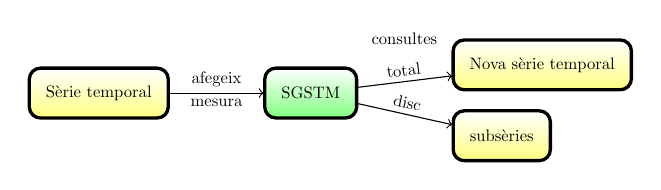
\begin{tikzpicture}[scale=0.6, every node/.style={transform shape}]

      \tikzset{
        mynode/.style={rectangle,rounded corners,draw=black, 
          very thick, inner sep=1em, minimum size=3em, text centered,
          groc},
        myarrow/.style={->, shorten >=1pt, thick},
        mylabel/.style={text width=7em, text centered},
        groc/.style={top color=white, bottom color=yellow!50},
        verd/.style={top color=white, bottom color=green!50},
        roig/.style={top color=white, bottom color=red!50},
      }  






 \node[mynode] (S) {Sèrie temporal};
 \node[mynode, verd, right=2cm of S] (sgstm) {SGSTM};
 \node[mynode, above right=-0.5cm and 2cm of sgstm] (Sp) {Nova sèrie temporal};
 \node[mynode, below=1.5cm of Sp.west, anchor=west] (S1) {subsèries};

 \draw[->] (S) -- (sgstm) node[above,midway,sloped] {afegeix} node[below,midway,sloped] {mesura}; 
 \draw[->] (sgstm) -- (Sp) node[above,midway,sloped] {total}; 
 \draw[->] (sgstm) -- (S1) node[above,midway,sloped] {disc}; 
 \node[left=2.1cm of Sp.north] (consultes) {consultes};

\end{tikzpicture}
\end{center}




Model d'operació de multiresolució (sobre un SGST):


\begin{center}
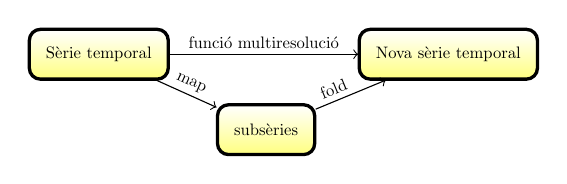
\begin{tikzpicture}[scale=0.6, every node/.style={transform shape}]

      \tikzset{
        mynode/.style={rectangle,rounded corners,draw=black, 
          very thick, inner sep=1em, minimum size=3em, text centered,
          groc},
        myarrow/.style={->, shorten >=1pt, thick},
        mylabel/.style={text width=7em, text centered},
        groc/.style={top color=white, bottom color=yellow!50},
        verd/.style={top color=white, bottom color=green!50},
        roig/.style={top color=white, bottom color=red!50},
      }  






 \node[mynode] (S) {Sèrie temporal};
 \node[mynode, right=4cm of S] (Sp) {Nova sèrie temporal};
 \draw[->] (S) -- (Sp) node[above,midway] {funció multiresolució}; 

 \node[mynode, below right=0.5cm and 1cm of S] (S1) {subsèries};
 \draw[->] (S) -- (S1) node[above,midway,sloped] {map}; 
 \draw[->] (S1) -- (Sp) node[above,midway,sloped] {fold\hphantom{mm}}; 


\end{tikzpicture}
\end{center}


\end{frame}




% \begin{frame}{Usos de la multiresolució}

% Possibilitats de computació:

%   \begin{itemize}
%   \item Computació offline
%   \item Computació incremental
%   \item Computació para\l.lela (offline)
%   \item Computació distribuïda (xarxes de sensors)
%   \end{itemize}


% Arquitectures dels sistemes:
%   \begin{itemize}

%   \item Únicament SGSTM: emmagatzematge amb pèrdua, aproximació a l'històric, dades originals no són necessàries.
%   \item SGST+SGSTM: dipòsit a llarg termini poc consultat i sistema per a resoldre consultes habituals o visualitzacions immediates
%   \item Funció de multiresolució (para\l.lela): experimentació 
%   \end{itemize}


% \end{frame}



\begin{frame}{Arquitectura dual}




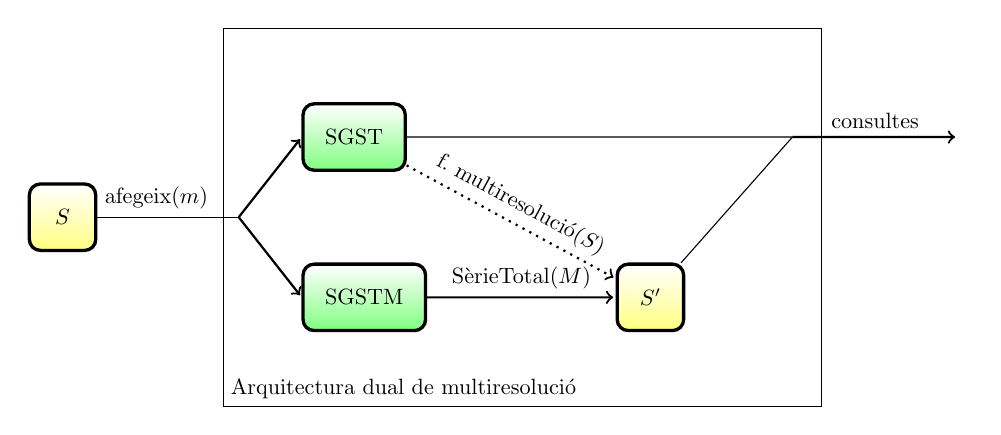
\begin{tikzpicture}[scale=0.8, every node/.style={transform shape}]

      \tikzset{
        mynode/.style={rectangle,rounded corners,draw=black, 
          very thick, inner sep=1em, minimum size=3em, text centered,
          groc},
        myarrow/.style={->, shorten >=1pt, thick},
        mylabel/.style={text width=7em, text centered},
        groc/.style={top color=white, bottom color=yellow!50},
        verd/.style={top color=white, bottom color=green!50},
        roig/.style={top color=white, bottom color=red!50},
      }  






 \node[mynode] (m) {$S$};

 \node[right=2cm of m] (mdins) {};

 \node[mynode, verd, above right=0.6cm and 1cm of mdins] (tsms) {SGST};

 \node[mynode, verd, below right=0.6cm and 1cm of mdins] (mtsms) {SGSTM};

 \node[rectangle,draw,minimum height=6cm,minimum width=9.5cm,right=-0.25cm of mdins] (dual) {};

\draw[shift=( dual.south west)]   
  node[above right] {Arquitectura dual de multiresolució};






 \node[mynode,right=3cm of mtsms] (ts) {$S'$};



 \draw (m.east) -- (mdins.east) node[above right,at start]
 {afegeix$(m)$};

 \draw[myarrow] (mdins.east) -- (tsms.west);
 \draw[myarrow] (mdins.east) -- (mtsms.west);


 \draw[myarrow, dotted] (tsms) -- (ts) node[above,midway,sloped]
 {f.~multiresolució$(S)$}; 
 
 \draw[myarrow] (mtsms) -- (ts) node[above,midway,sloped]
 {SèrieTotal$(M)$};




 \node[right=6cm of tsms] (consdins) {};

 \draw (tsms) -- (consdins.center);
 \draw (ts) -- (consdins.center);

 \node[right=2.5cm of consdins] (consultes) {};
 \draw[myarrow] (consdins.center) -- (consultes) node[above,midway,sloped]
 {consultes};



\end{tikzpicture}

Conceptes relacionats: 
\begin{itemize}
\item Arquitectura Lambda \parencite{marz14:bigdata} 
\item Precomputació de vistes \parencite{date04:introduction8}
\end{itemize}





\end{frame}




\subsection*{Teoria de la informació}
\begin{frame}{Sobre la qualitat de la multiresolució}

  Quantificació de l'error que es comet en la selecció de la informació
  per a la multiresolució:

\begin{center}
consulta(sèrie temporal original) vs.\ consulta(multiresolució)
\end{center}


Alguns dels escenaris particulars analitzats:
\begin{itemize}
\item Consulta a tota la sèrie temporal i mateixa consulta i atribut:
  \begin{itemize}
  \item Màxim i total no tenen error
  \item Mitjana té error
  \item Mitjana en el cas d'una sèrie temporal regular no té error 
  \end{itemize}

\item Consultes d'un interval determinat:
  \begin{itemize}
  \item Interval múltiple de les resolucions consolidades: similar al punt anterior
  \item No múltiple: hi ha error. Fitat per a variables monòtones creixents.
  \end{itemize}

% \item Conservació dels totals en comptadors

% \item Equivalència de l'atribut mitjana en sèries temporals regulars per a diversos mètodes de representació.

\end{itemize}

\end{frame}




%%% Local Variables: 
%%% mode: latex
%%% TeX-master: "defensa"
%%% End: 
%  LocalWords:  multiresolució



\section{Conclusions}
\begin{frame}{Conclusions}
\end{frame}

\begin{frame}{Treball futur}
\end{frame}



%%% Local Variables: 
%%% mode: latex
%%% TeX-master: "defensa"
%%% End: 


\begin{frame}<handout:0>
  \addtocounter{framenumber}{-1}

  \begin{center}
    {\huge
      Gràcies per l'atenció!
    }
  \end{center}

\end{frame}


\appendix


\begin{frame}[allowframebreaks]{Referències}

\printbibliography

\end{frame}


\end{document}


%%%%%%%%%%%%%%%%%%%%%%%%%%%%%%%%%%%%%%%%%%%%%%%%%%%%%%%%%%%%%%%%%%%%%%%%%%  
% Defensa Tesi Doctoral. 
%
% Copyright (C) 2011-2015 Aleix Llusà Serra.
% 
% This LaTeX document is free software: you can redistribute it and/or
% modify it under the terms of the GNU General Public License as
% published by the Free Software Foundation, either version 3 of the
% License, or (at your option) any later version.
%
% This document is distributed in the hope that it will be useful, but
% WITHOUT ANY WARRANTY; without even the implied warranty of
% MERCHANTABILITY or FITNESS FOR A PARTICULAR PURPOSE. See the GNU
% General Public License for more details.
%
% You should have received a copy of the GNU General Public License
% along with this document. If not, see <http://www.gnu.org/licenses/>.
%
%
% Aleix Llusà Serra
% Departament de Disseny i Programació de Sistemes Electrònics de la Universitat Politècnica de Catalunya (DiPSE-UPC)
% Escola Politècnica Superior d'Enginyeria de Manresa (EPSEM)
% Av. de les Bases de Manresa, 61-73
% 08242 Manresa (Barcelona)
% PAÏSOS CATALANS 
%
% aleix (a) dipse.upc.edu
% 
% El codi font LaTeX del document es troba a 
% <http://escriny.epsem.upc.edu/projects/rrb/>
%%%%%%%%%%%%%%%%%%%%%%%%%%%%%%%%%%%%%%%%%%%%%%%%%%%%%%%%%%%%%%%%%%%%%%%%%% 